% Options for packages loaded elsewhere
\PassOptionsToPackage{unicode}{hyperref}
\PassOptionsToPackage{hyphens}{url}
%
\documentclass[
  12pt,
]{article}
\usepackage{amsmath,amssymb}
\usepackage{lmodern}
\usepackage{iftex}
\ifPDFTeX
  \usepackage[T1]{fontenc}
  \usepackage[utf8]{inputenc}
  \usepackage{textcomp} % provide euro and other symbols
\else % if luatex or xetex
  \usepackage{unicode-math}
  \defaultfontfeatures{Scale=MatchLowercase}
  \defaultfontfeatures[\rmfamily]{Ligatures=TeX,Scale=1}
  \setmainfont[]{Times New Roman}
\fi
% Use upquote if available, for straight quotes in verbatim environments
\IfFileExists{upquote.sty}{\usepackage{upquote}}{}
\IfFileExists{microtype.sty}{% use microtype if available
  \usepackage[]{microtype}
  \UseMicrotypeSet[protrusion]{basicmath} % disable protrusion for tt fonts
}{}
\makeatletter
\@ifundefined{KOMAClassName}{% if non-KOMA class
  \IfFileExists{parskip.sty}{%
    \usepackage{parskip}
  }{% else
    \setlength{\parindent}{0pt}
    \setlength{\parskip}{6pt plus 2pt minus 1pt}}
}{% if KOMA class
  \KOMAoptions{parskip=half}}
\makeatother
\usepackage{xcolor}
\usepackage[margin=2.54cm]{geometry}
\usepackage{graphicx}
\makeatletter
\def\maxwidth{\ifdim\Gin@nat@width>\linewidth\linewidth\else\Gin@nat@width\fi}
\def\maxheight{\ifdim\Gin@nat@height>\textheight\textheight\else\Gin@nat@height\fi}
\makeatother
% Scale images if necessary, so that they will not overflow the page
% margins by default, and it is still possible to overwrite the defaults
% using explicit options in \includegraphics[width, height, ...]{}
\setkeys{Gin}{width=\maxwidth,height=\maxheight,keepaspectratio}
% Set default figure placement to htbp
\makeatletter
\def\fps@figure{htbp}
\makeatother
\setlength{\emergencystretch}{3em} % prevent overfull lines
\providecommand{\tightlist}{%
  \setlength{\itemsep}{0pt}\setlength{\parskip}{0pt}}
\setcounter{secnumdepth}{5}
\ifLuaTeX
  \usepackage{selnolig}  % disable illegal ligatures
\fi
\IfFileExists{bookmark.sty}{\usepackage{bookmark}}{\usepackage{hyperref}}
\IfFileExists{xurl.sty}{\usepackage{xurl}}{} % add URL line breaks if available
\urlstyle{same} % disable monospaced font for URLs
\hypersetup{
  pdftitle={Data analysis},
  pdfauthor={PengYangYu},
  hidelinks,
  pdfcreator={LaTeX via pandoc}}

\title{Data analysis}
\author{PengYangYu}
\date{2022-11-14}

\begin{document}
\maketitle

\hypertarget{research-question-1}{%
\subsubsection{Research question 1:}\label{research-question-1}}

Is there any correlation between ozone concentration and daily AQI in
2022?

The null hypothesis: ozone concentration has no correlation with daily
AQI

The alternative hypothesis: ozone concentration has correlation with
daily AQI

\begin{verbatim}
## `geom_smooth()` using formula 'y ~ x'
\end{verbatim}

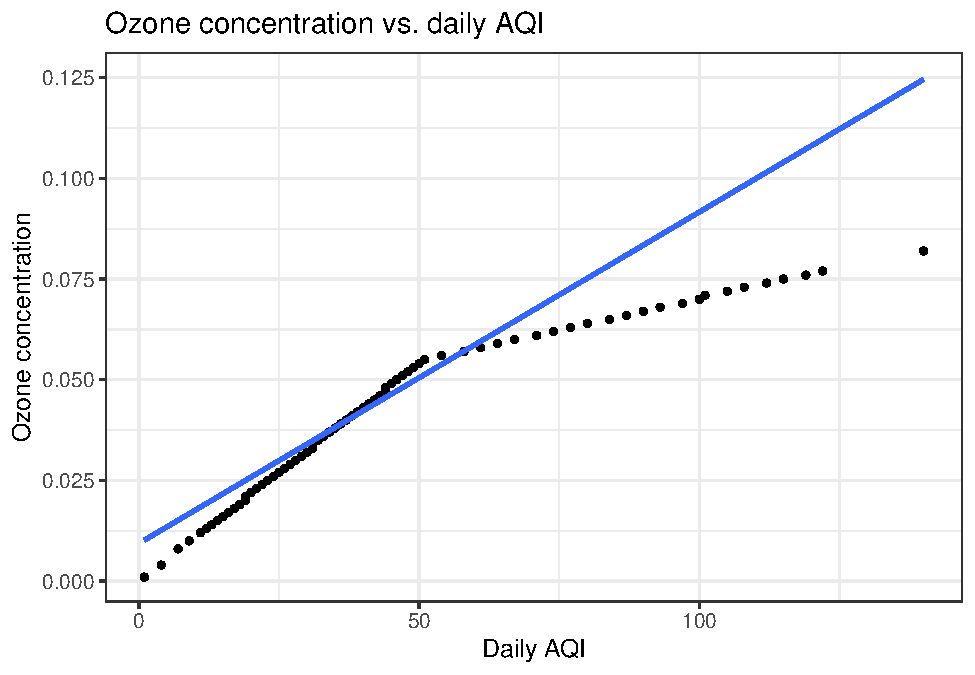
\includegraphics{Project_DataAnalysis_files/figure-latex/Q1 Linear regression-1.pdf}

\begin{verbatim}
## 
## Call:
## lm(formula = Concentration ~ DailyAQI, data = EPAair_O3_22)
## 
## Residuals:
##       Min        1Q    Median        3Q       Max 
## -0.042585 -0.000866  0.000372  0.001434  0.003672 
## 
## Coefficients:
##              Estimate Std. Error t value Pr(>|t|)    
## (Intercept) 9.350e-03  1.110e-04   84.25   <2e-16 ***
## DailyAQI    8.231e-04  2.688e-06  306.23   <2e-16 ***
## ---
## Signif. codes:  0 '***' 0.001 '**' 0.01 '*' 0.05 '.' 0.1 ' ' 1
## 
## Residual standard error: 0.002882 on 9287 degrees of freedom
## Multiple R-squared:  0.9099, Adjusted R-squared:  0.9099 
## F-statistic: 9.378e+04 on 1 and 9287 DF,  p-value: < 2.2e-16
\end{verbatim}

The R-squared of this linear model is 0.9099, which means that 90.99\%
variability in daily air quality index (AQI) is explained by changes in
ozone concentration. The degrees of freedom of the model is 9287 =
9289-2 since the number of observations is 9289 and the number of
parameters is 2. According to the p-value of slope, which is smaller
than 0.05, we reject the null hypothesis, so the correlation between
ozone concentration and daily AQI in 2022 is significant.

\hypertarget{research-question-2}{%
\subsubsection{Research question 2:}\label{research-question-2}}

Do different sites have equal mean of ozone concentrations in 2022?

The null hypothesis: they have equal mean of concentrations

The alternative hypothesis: they do not have equal mean of
concentrations

\begin{verbatim}
## [1] "There are 38 sites in total and 28 of them follow a normal distribution."
\end{verbatim}

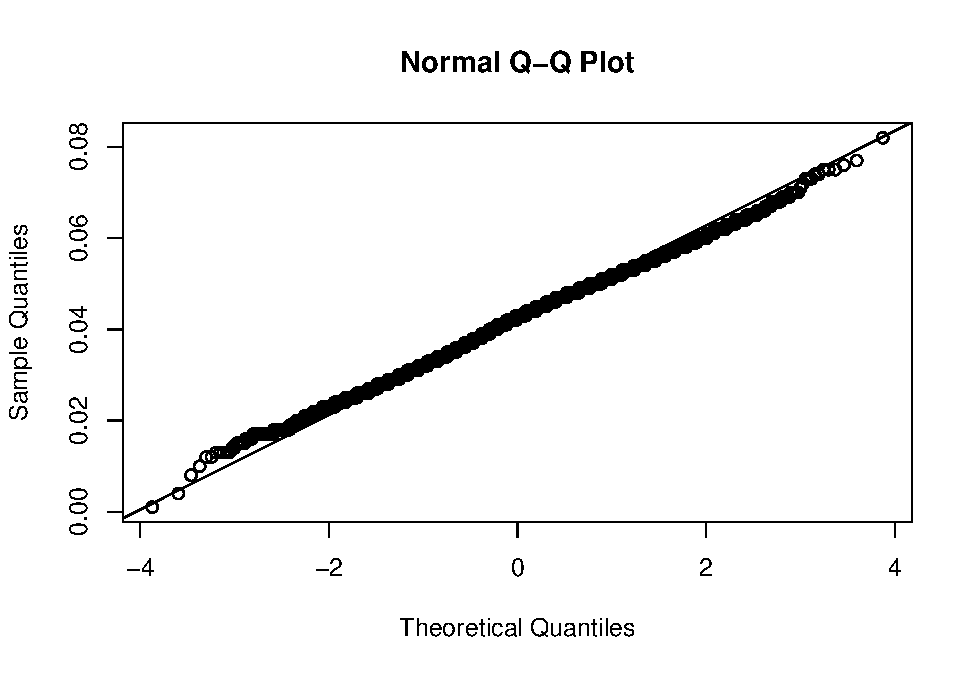
\includegraphics{Project_DataAnalysis_files/figure-latex/Q2 ANOVA-1.pdf}

\begin{verbatim}
## 
##  Bartlett test of homogeneity of variances
## 
## data:  EPAair_O3_22$Concentration and EPAair_O3_22$SiteName
## Bartlett's K-squared = 114.06, df = 37, p-value = 8.769e-10
\end{verbatim}

\begin{verbatim}
##               Df Sum Sq   Mean Sq F value Pr(>F)    
## SiteName      37 0.0546 0.0014746   17.02 <2e-16 ***
## Residuals   9251 0.8016 0.0000867                   
## ---
## Signif. codes:  0 '***' 0.001 '**' 0.01 '*' 0.05 '.' 0.1 ' ' 1
\end{verbatim}

From the Shapiro-Wilk test result and normal Q-Q plot, we find that most
of the sites are conform to normal population distribution assumption.
However, the Bartlett's test result shows that the null hypothesis that
the variances in each sites are the same is rejected. Since ANOVA is
robust against departures from equal variance, we can still apply
one-way ANOVA on our dataset.

The p-value of the ANOVA is smaller than 0.05, so we reject the null
hypothesis. Therefore, the mean of ozone concentrations in 2022
significantly differ among sites.

\hypertarget{research-question-3}{%
\subsubsection{Research question 3:}\label{research-question-3}}

Is the mean of ozone concentrations in 2021 and 2022 equivalent?

The null hypothesis: the mean between 2021 and 2022 is equivalent

The alternative hypothesis: the mean between 2021 and 2022 is not
equivalent

\begin{verbatim}
## `stat_bin()` using `bins = 30`. Pick better value with `binwidth`.
\end{verbatim}

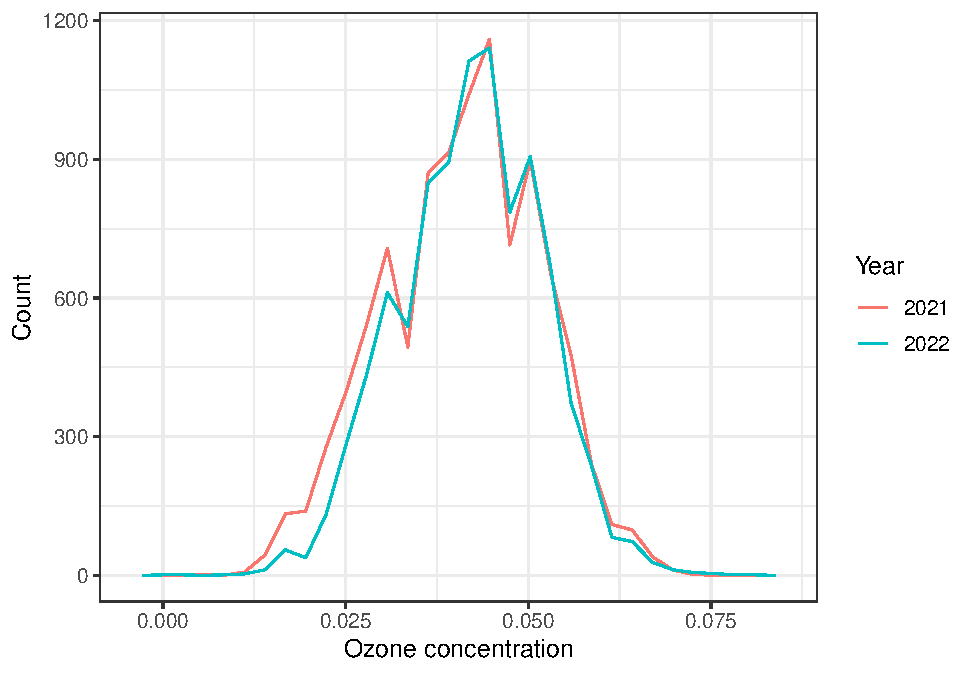
\includegraphics{Project_DataAnalysis_files/figure-latex/Q3 T-test-1.pdf}
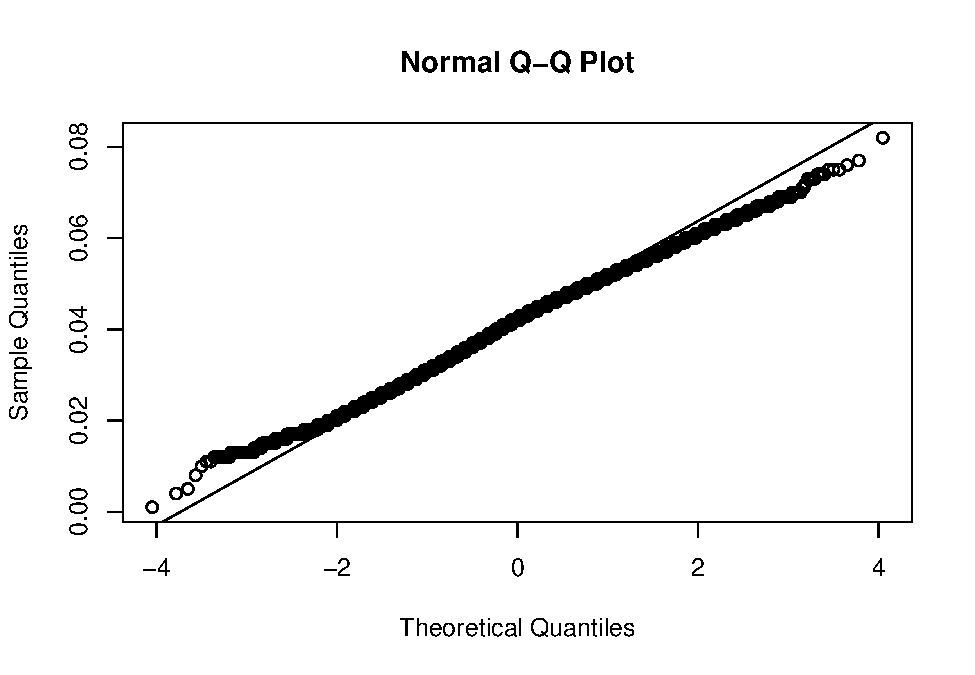
\includegraphics{Project_DataAnalysis_files/figure-latex/Q3 T-test-2.pdf}

\begin{verbatim}
## 
##  Bartlett test of homogeneity of variances
## 
## data:  EPAair_O3_2122$Concentration and EPAair_O3_2122$Year
## Bartlett's K-squared = 103.52, df = 1, p-value < 2.2e-16
\end{verbatim}

\begin{verbatim}
## 
##  Welch Two Sample t-test
## 
## data:  Concentration by Year
## t = -7.0983, df = 19249, p-value = 1.307e-12
## alternative hypothesis: true difference in means between group 2021 and group 2022 is not equal to 0
## 95 percent confidence interval:
##  -0.0013217999 -0.0007497675
## sample estimates:
## mean in group 2021 mean in group 2022 
##         0.04104097         0.04207676
\end{verbatim}

The normal Q-Q plot shows that the data has small deviations from normal
distribution. The Bartlett's test result shows that the variances
between 2021 and 2022 are different. Again, t-test is robust to these.
The T-test suggests that the mean of ozone concentrations in 2021 and
2022 is not equivalent with p-value smaller than 0.05.

\hypertarget{research-question-4}{%
\subsubsection{Research question 4:}\label{research-question-4}}

Is there any trend of ozone concentrations in space?

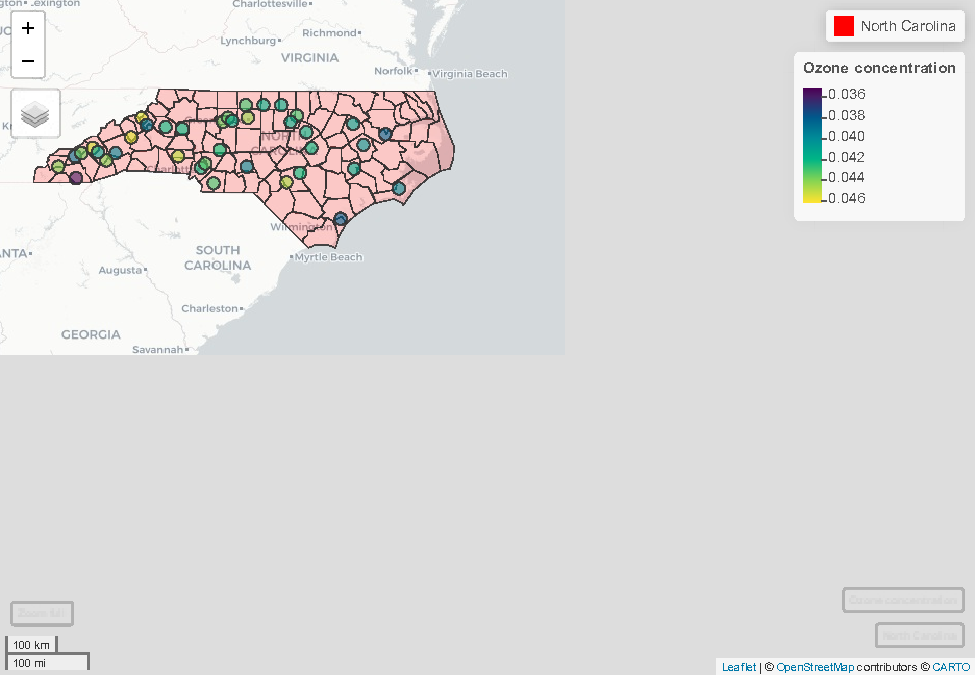
\includegraphics{Project_DataAnalysis_files/figure-latex/Q4 Spatial analysis-1.pdf}
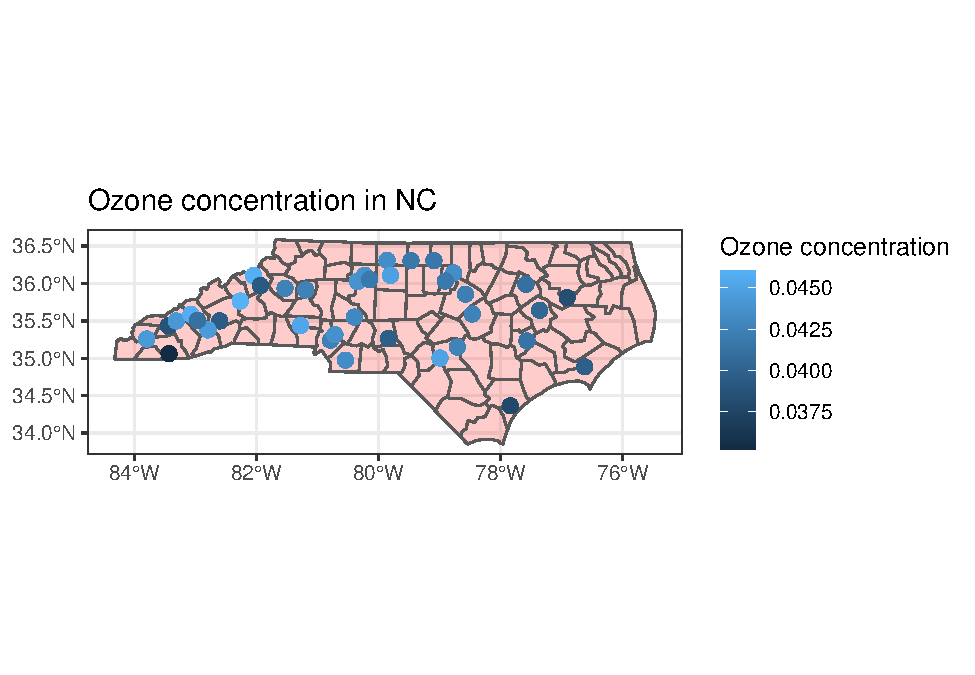
\includegraphics{Project_DataAnalysis_files/figure-latex/Q4 Spatial analysis-2.pdf}

It seems there is no obvious trend between the location of sites and the
mean ozone concentration collected from the sites.

\hypertarget{research-question-5}{%
\subsubsection{Research question 5:}\label{research-question-5}}

Have ozone concentrations changed from 2016 to 2022 at Rockwell?

The null hypothesis: the ozone concentration is stationary over time

The alternative hypothesis: the ozone concentration change over time

\begin{verbatim}
## `geom_smooth()` using formula 'y ~ x'
\end{verbatim}

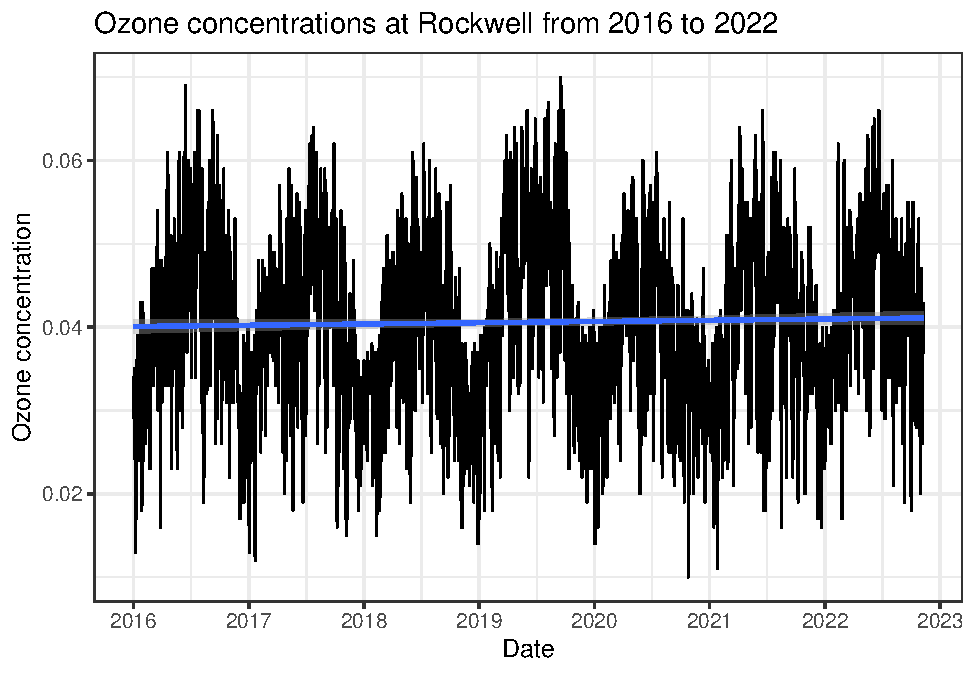
\includegraphics{Project_DataAnalysis_files/figure-latex/Q5 Time series analysis-1.pdf}
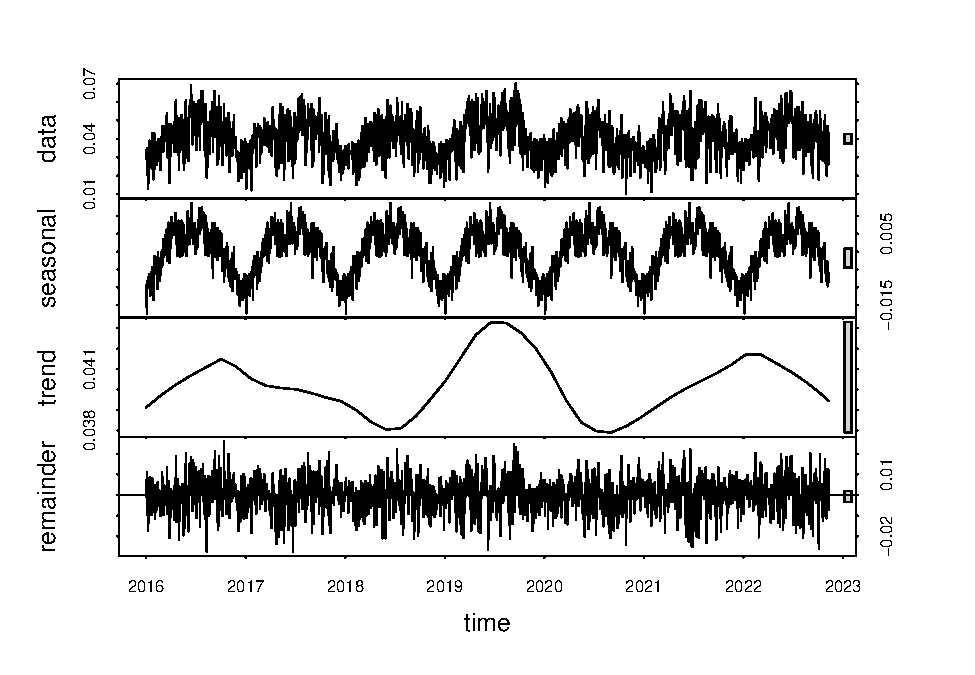
\includegraphics{Project_DataAnalysis_files/figure-latex/Q5 Time series analysis-2.pdf}

\begin{verbatim}
## Score =  87 , Var(Score) = 15119
## denominator =  7239.089
## tau = 0.012, 2-sided pvalue =0.47922
\end{verbatim}

The Seasonal Mann-Kendall test is chosen to test monotonic trend because
the decomposed figure shows that the time series object has a strong
seasonal component. From the result, we accept the null hypothesis since
the p-value is greater than 0.05. Therefore, the ozone concentration at
Rockwell is stationary from 2016 to 2022.

\end{document}
